\chapter{Introducción}


\section{Descripción General}



\section{Objetivos}
\subsection{Objetivo General}

Implementar un system on chip OpenSource con un microprocesador embebido
Soft-core que soporte un sistema operativo libre , con la finalidad de entregar
un sitema integral FPGA-SoC-Sistema Operativo completamente funcional y bajo licencia GPL v2.

\subsection{Objetivo Especìfico}
\begin{itemize}
\item Seleccionar, analizar y determinar un microprocesador Soft-Core.
\item Establecer un system on chip Open Source donde poder implementar un Soft-Core.
\item Determinar sistemas operativo con licencia GPL v2 que tengan las prestaciones funcionales adecuadas.
\end{itemize}

\section{Motivación} 

Existe un grupo de cores Soft-Core de código abierto que no están limitados por la tecnología. Los cores destacados de microprocesadores de 32 bits,
son los procesadores SPARC LEON OpenRISC 1200 , y el core de LatticeMico32. Usar cores de  código abierto,  va unido a una serie de conceptos como:
 \begin {itemize}
\item
\textit{Flexibilidad}  Si el código fuente está disponible, los desarrolladores pueden modificar el codigo de acuerdo a sus necesidades. Además, se
produce un flujo constante de ideas que mejora la calidad del código.
\item 
\textit{Fiabilidad y seguridad}  Con muchos programadores a la vez escrutando el mismo trabajo, los errores se detectan y corrigen antes, por lo que
el producto resultante es mas fiable y eficaz que el comercial.
\item 
\textit{Rapidez de desarrollo}  Las actualizaciones y ajustes se realizan a través de una comunicación constante vía Internet.
\item 
\textit{Relación con el usuario} El programador se acerca mucho mas a las necesidades reales de su cliente, y puede crear un producto especifico para
él
 \end {itemize}
 
Obtener un sistema integral de código abierto en donde se tiene código HDL, assembler y C disponible para adaptarse de acuerdo a los requerimientos del proyecto. Ademas de la de la capacidad de migrar de una plataforma a otra. Logrando menor dependencia entre el código fuente y la plataforma objetivo. 
La portabilidad del código abierto nos permite implementarlo sobre una ASICs (Application-specific integrated circuit) o con modificaciones menores en cualquier FPGA (Field Programmable Gate Array) de Xilinx, Altera, Lattice, etc. 
Estos tres de los más grandes proveedores de FPGA , Xilinx , Altera y Lattice , ofrecen sus propios micro core RISC de 32bits los dos mayores proveedores de dispositivos FPGA , Altera y Xilinx , proporcionan el micro core Nios y Microblaze, respectivamente. Son micro cores  en donde el código fuente RTL no se encuera disponible y solo pueden ser implementados en sus respectivas FPGA.

\section{Metodologìa}

El modelo de desarrollo a utilizar es el Modelo en Espiral tipificado por Ian Sommerville\cite{Etiqueta00} . El modelo en espiral de ingeniería de software, mostrado en la Ilustración 1, fue originalmente propuesto por Boehm en año 1988, en su artículo A Spiral Model of Software Development and Enhancement. Propuso un marco del proceso de software dirigido por el riesgo. Aquí, el proceso de software se representa como una es espiral, cada ciclo en la espiral representa una fase del proceso de software. Por ende el, ciclo más interno puede relacionarse con la factibilidad del sistema, el siguiente ciclo con la definición de requerimientos, el siguiente ciclo al diseño del sistema, y así sucesivamente.


\begin{figure}[h!]
 \begin{center}
  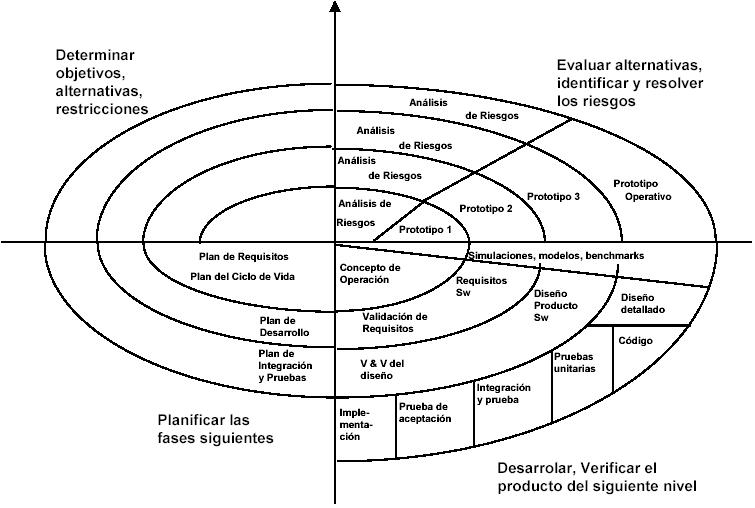
\includegraphics[width=1\textwidth,keepaspectratio=true]{./images/ESPIRAL}
  \caption{Arquitectura MinSoc}
  \label{fig:esquema}
 \end{center}
\end{figure}


Cada ciclo del espiral se divide en 4 sectores:
 
\begin {itemize}
\item 
\textit{Establecimiento de objetivo}  Se definen objetivos específicos para dicha fase del proyecto. Se identifican restricciones en el preceso y el producto, y se traza un plan detallado de gestión. Se identifican los riesgos del proyecto. Dependiendo de estos riegos, se planean estrategias alternativas
\item 
\textit{Validación y reducción del riesgo}  En cada uno de los riesgos identificados del proyecto, se realiza un análisis minucioso. Se dan acciones para reducir el riesgo.
\item 
\textit{Desarrollo y validación}  Despues de una evaluacion del riesgo, se elige un modelo de desarrollo para el sistema.
\item 
\textit{Planeción}  El proyecto se revisa y se toma una decisión sobre si hay que continuar con otro ciclo de la espiral. Si se opta por continuar, se trazan los planes para la siguente fase del proyecto.
 \end {itemize}

Como característica principal de esta metodología es que posee una consideración explícita del riesgo. Informalmente, el riesgo significa sencillamente que algo puede ir mal. Los riegos originan problemas en el proyecto, como los de confección de agendas y excesos en los costos; por lo tanto, la disminución de riegos es una actividad sumamente importante en la gestión del proyecto.
Un ciclo en la espiral comienza con la elaboración de objetivos, como el rendimiento y la funcionalidad. Entonces se enumeran formas alternativas de alcanzar estos objetivos y las restricciones impuestas en cada una de ellas. Cada alternativa se evalúa contra cada objetivo y se identifican las fuentes de riegos del proyecto. El siguiente paso es resolver estos riesgos mediante actividades de recopilación de información como la de detallar más el análisis, la construcción de prototipos y la simulación. Una vez que se han evaluado los riesgos se llevará a cabo cierto desarrollo, seguido de una actividad de planificación para la siguiente fase del proceso.


\section{Importancia del Problema}

En el diseño del sistema embebido se usan diferentes procesos depende del tipo de sistema, el hardware disponible y la organización que desarrolle el sistema. Una de las actividades principales en un proceso de diseño de software es la elección del hardware y del sistema operativo que se efectúa antes del comienzo del software. Ante tal situación , se debe diseñar el software par considerar las restricciones impuestas por las capacidades del hardware.
Los efectos que influyen dichas elecciones comprenden restricciones de de temporización sobre el sistema, limitación en la energía disponible, experiencia del equipo de desarrollo y limites en el costos del sistema entregable.
 
Se está explorando una linea donde se busca dar al diseñador del sistema embebido una solución flexible en la primera etapa de la elección de plataforma. Donde a través del análisis de diferentes plataformas de desarrollo OpenSource y privativas pueda elegir la mejor opción para el tipo de sistema a desarrollar y requerimientos de proceso. 
 
Una vez que se ha elegido la plataforma de ejecucion para el sistema, se ha diseñado una arquitectura de proceso y se a determinado una políticas de planeación, es necesario comprobar que el sistema cumplirá sus con sus requerimientos.

%El softcore OpenRisc  que se encuentra en el SoC OrpSoc y MinSoc se tiene que implementado en una FPGA  Spartan 3A de Xilinx. Tenemos como fin montar un Linux para validar y verificar el sistema global entregando un sistema funcional bajo licencia libre.
%Actualmente las FPGAs nos birndan la posibilidad de implementar estos proyectos, donde el Hardware y el Software son una misma entidad. Este nuevo enfoque nos permite aprovechar la facilidad de implementar soluciones por Hardware.

\section{Alcance de Estudio}
\section{Modelo de Desarollo}
\section{Metodologìa}




%%%%% poner en negrita asi \textit{Python} 


